We propose a framework that allows end-users to teach a robot a goal-oriented behaviour and consisting of the following three steps (\fig{fig:framework}): 
\begin{enumerate}
	\item[A.]{Programming by Demonstration: user demonstrates atomic actions and teaches symbolic action models, in terms of preconditions and effects.}
	\item[B.]{Automated Planning: robot uses action models to generate an action sequence to achieve a goal.}
	\item[C.]{Retro-active Loop: user refines the learned action models in case of ambiguities.}
\end{enumerate}
In the following sections, we discuss each step in more detail. 
%We refer the reader to a video of the framework: \texttt{https://youtu.be/DTm2YjiSNQM}
%Using this knowledge base, the user can define a planning problem, for which the robot will generate a plan. 

\begin{figure}[!h]
	\centering
	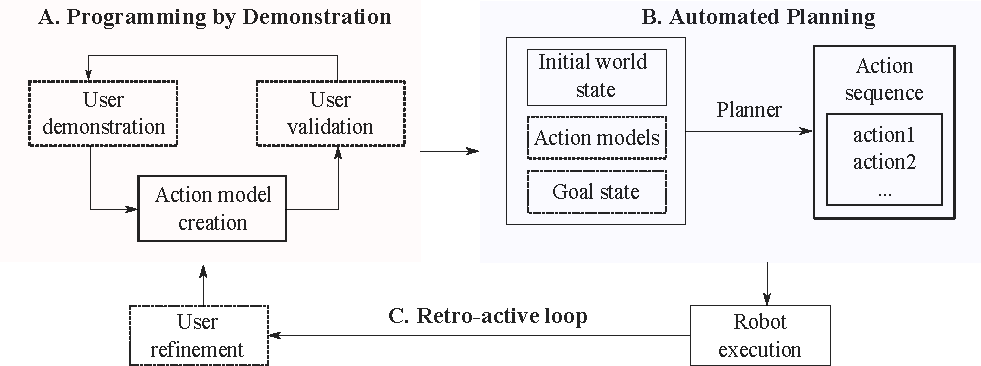
\includegraphics[width=\linewidth]{figures/framework}
	\caption{A robot programming framework for non-expert users: the user teaches action models, which are used by the robot with an automated planner, to generate an action sequence to achieve a goal.
After an unsuccessful robot execution, the user can refine the taught action models (dotted lines indicate user actions, solid lines indicate robot actions).}
	\label{fig:framework}
\end{figure}

\section{Programming by Demonstration: teaching action models}
Programming by demonstration (PbD) techniques generally consist of an iterative process.
The user demonstrates an atomic action, such as moving a cube from an initial position A to a final position B \texttt{(move cube A B)}.
An action execution results in a change in the world state, such as the cube's position.
The robot observes the changes before and after the action demonstration (Fig. \ref{fig:action} top), and extracts the relevant preconditions and effects to build a generalised action model, expressed in a symbolic planning language (Fig. \ref{fig:action} bottom).
The user validates the learned action model, and provides additional demonstrations if necessary.

The robot learns from multiple demonstrations to generalise trajectories and high-level conditions.
In the framework, we assume that the learned action trajectory is independent of the trajectory performed by the teacher.
Dynamic Movement Primitives (DMP) can cope with the generalisation of a demonstrated trajectory \cite{pastor2009learning}.
To learn high-level conditions, the robot uses a perception system (e.g. SIFT \cite{ahmadzadeh2015learning} or a database of object features \cite{mason2011robot}) that recognises object properties in the state of the world. 
%Note that we do not address the perception problem in this paper. 
In our experiments, we implemented a simple python algorithm with integrated functionalities of the Robot Operating System (ROS), to detect and move objects, based on their colour.

Feature-based algorithms, such as k-means clustering \cite{mollard2015robot}, can be used to generalise over high-level conditions.

%Table \ref{tab:action-model} shows the states of the demonstrated action and the generalised action model. 
%The generalised operator is automatically translated into a symbolic representation, allowing the creation of a planning domain, without the need for any programming knowledge.

Existing PbD approaches try to teach the robot from a small number of demonstrations \cite{orendt2016robot,abdo2013learning}.
We propose an interactive learning approach, where the user can directly modify the learned action models using a user-interface.


\section{Automated Planning: using action models}\label{sec:AP}
The robot uses the learned symbolic action models in combination with an automated planner to achieve user-defined goals. 
%Automated planners try to model the robot's strategies, when operating in diverse environments \cite{ghallab2004automated}.
The initial world state is automatically recognised by the robot using the same perception system as in the PbD phase. 
%The automated planner generates a plan, consisting of an ordered action sequence for the robot to execute. 
The user can change the initial object configuration of the world state, and enter an arbitrary goal, that can be achieved using the taught action models.
If the user changes the goal, a new action sequence is generated by the planner.
Generating a plan under different initial states allows the user to test the created action models.
There exist various planners that can be used for symbolic planning with robots: Metric-FF (\cite{cubek2015high}), or a fast downward planner (\cite{abdo2013learning}). 


\section{Retro-active Loop: refining action models}
The execution to a new context is an important step to test the taught action models.
It is likely that the execution of the plan does not produce the desired outcome, especially if the plan is executed in a context different to the demonstration (e.g. different object colour or position).
Missing preconditions or effects for an action model can lead to suboptimal or non-existing solutions and will need to be corrected by the user.
The retro-active loop allows the user to revisit the created action models.
Knowledge engineering tools (\sect{subsec:Knowledge Engineering}) provide a user-interface to facilitate this process of modifying action models used for automated planners.
They often provide useful functionalities for dynamic testing, model checking and visualisation (\cite{simpson2007planning}), where the quality of the models generated does not depend on the user's expertise.
